\iffalse
\let\negmedspace\undefined
\let\negthickspace\undefined
\documentclass[journal,12pt,twocolumn]{IEEEtran}
\usepackage{cite}
\usepackage{amsmath,amssymb,amsfonts,amsthm}
\usepackage{algorithmic}
\usepackage{graphicx}
\usepackage{textcomp}
\usepackage{xcolor}
\usepackage{txfonts}
\usepackage{listings}
\usepackage{enumitem}
\usepackage{mathtools}
\usepackage{gensymb}
\usepackage{comment}
\usepackage[breaklinks=true]{hyperref}
\usepackage{tkz-euclide} 
\usepackage{listings}
\usepackage{gvv}                                        
\def\inputGnumericTable{}                                 
\usepackage[latin1]{inputenc}                                
\usepackage{color}                                            
\usepackage{array}                                            
\usepackage{longtable}                                       
\usepackage{calc}                                             
\usepackage{multirow}                                         
\usepackage{hhline}                                           
\usepackage{ifthen}                                           
\usepackage{lscape}

\newtheorem{theorem}{Theorem}[section]
\newtheorem{problem}{Problem}
\newtheorem{proposition}{Proposition}[section]
\newtheorem{lemma}{Lemma}[section]
\newtheorem{corollary}[theorem]{Corollary}
\newtheorem{example}{Example}[section]
\newtheorem{definition}[problem]{Definition}
\newcommand{\BEQA}{\begin{eqnarray}}
\newcommand{\EEQA}{\end{eqnarray}}
\newcommand{\define}{\stackrel{\triangle}{=}}
\theoremstyle{remark}
\newtheorem{rem}{Remark}
\begin{document}
\bibliographystyle{IEEEtran}
\vspace{3cm}
\title{NCERT DISCRETE 11.9.5 Q9}
\author{EE23BTECH11214 - Harsha Vardhan Kumar$^{*}$% <-this % stops a space
}
\maketitle
\newpage
\bigskip
\textbf{Question}:\\
The first term of a G.P. is $1$. The sum of the third term and fifth
term is $90$. Find the common ratio of G.P.
\\
\solution\\
\fi
\begin{table}[htbp]
\centering
\begin{tabular}{|l|l|c|}
\hline
\textbf{Symbol} & \textbf{Description} & \textbf{Value} \\
\hline
$x\brak{n}$ & General term & $ar^n$ \\
\hline
$a$ & First term & 1 \\
\hline
$r$ & Common ratio & - \\
\hline
$x\brak{2} + x\brak{4}$ & Sum of 3rd and 5th terms & 90 \\
\hline
\end{tabular}

\caption{Given parameters list}
\end{table}
\begin{align}
ar^2 + ar^4 &= 90 \\
r^2 + r^4 &= 90 \\
\brak{r^2 - 9}\brak{r^2 + 10} &= 0 \\
r^2 &= 9 \\
r &= \pm 3
\end{align}
From  \eqref{eq:GPsum} \\
For $r = 3$
\begin{align}
X\brak{z} = \frac{1}{1 - 3z^{-1}}  , \quad \abs{z} > \abs{3}
\end{align}
For $r = -3$
\begin{align}
X\brak{z} = \frac{1}{1 + 3z^{-1}}  , \quad \abs{z} > \abs{-3}
\end{align}
\begin{figure}
   \centering
     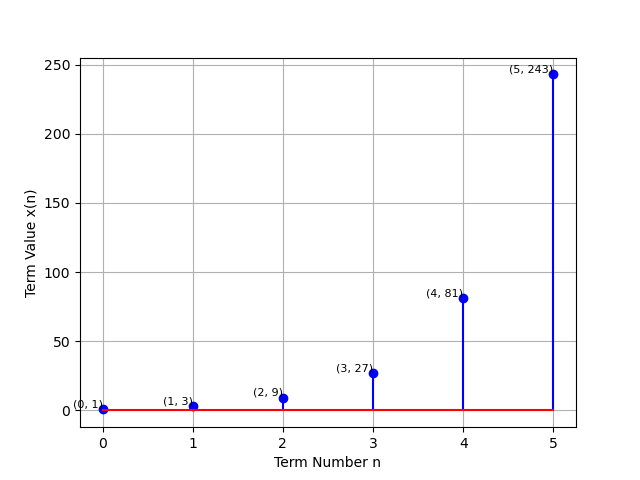
\includegraphics[width=1\columnwidth, height=1\columnwidth]{ncert-maths/11/9/5/9/figs/graph.png}
     \caption{r = 3}
\end{figure}
\begin{figure}
   \centering
     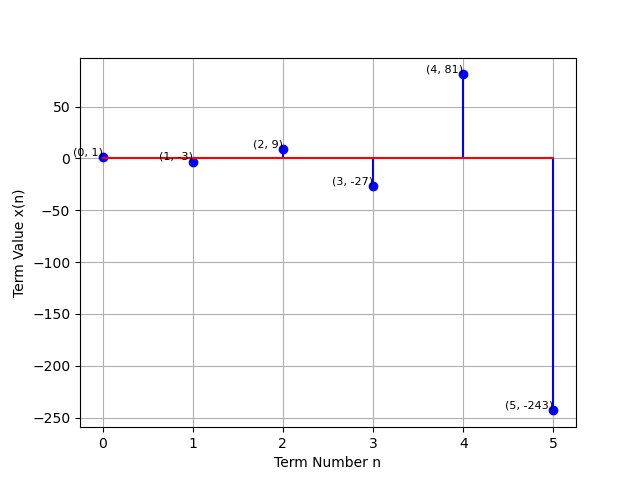
\includegraphics[width=1\columnwidth, height=1\columnwidth]{ncert-maths/11/9/5/9/figs/graph1.png}
     \caption{r = -3}
\end{figure}
%\end{document}
